\subsection{ABBA expanded to Team Games}

\subsubsection{2vs2}

\paragraph{2vs2: ABBA in Orders and determining Move Order}

Team Games (2vs2s and 3vs3s) tend to have cyclic move order. Expanding on this, the order follows the same ABBA pattern. In a 2vs2 game between Team A (players A1 and A2) and Team B (players B1 and B2), the move order would follow the pattern $$\text{A1,B1,B2,A2} ,\text{A2,B2,B1,A1} , \text{A1,B1,B2,A2} \dots$$

This is best illustrated in the Figure \ref{moveorder_2v2s}. Also remember that the ABBA pattern follows both the moves - orders and the deployments.

\begin{figure}[H]
  \centering
  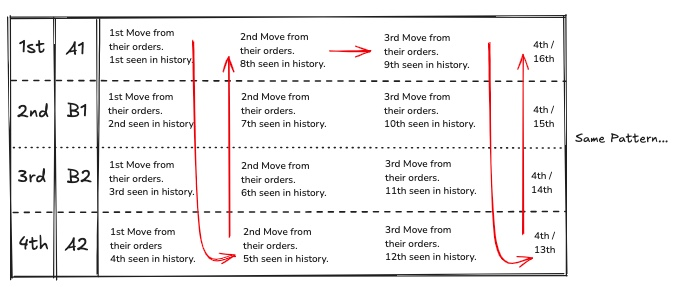
\includegraphics[width=\textwidth]{Images/moveorder2v2.jpg}
  \caption{Move Order in 2vs2 games}
  \label{moveorder_2v2s}
\end{figure}

For example, in this \href{https://www.warzone.com/MultiPlayer?GameID=37917076}{Strategic 2vs2} game when checking the history from everyone's POV as well as my POV after Turn 1 we see Figure \ref{ex1} and \ref{ex2}.

\begin{figure}[H]
  \centering
  \begin{minipage}[b]{0.48\linewidth}
    \centering
    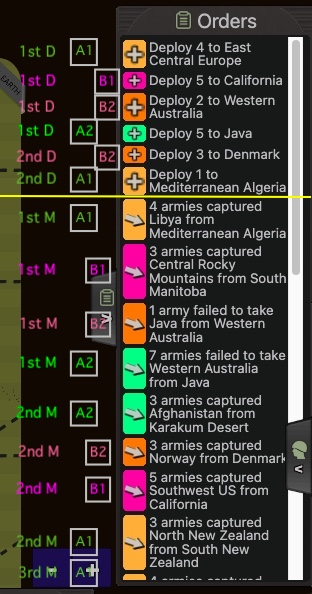
\includegraphics[width=\linewidth, height=13cm]{Images/ex1.jpg}
    \caption{Full POV}
    \label{ex1}
  \end{minipage}
  \hfill
  \begin{minipage}[b]{0.48\linewidth}
    \centering
    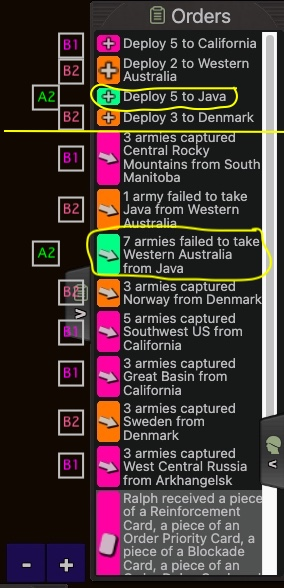
\includegraphics[width=\linewidth, height=13cm]{Images/ex2.jpg}
    \caption{My Perspective}
    \label{ex2}
  \end{minipage}
\end{figure}

After Turn 1 me and my teammate should be able to figure out the move order within seconds. Upon seeing history, it's straight forward that on Turn 1 the order is Ralph->7ate9, with Xeno making an attack visible to us in between 7ate9's 1st and 2nd move. If Xeno and Jack were team B, then the moves we see in history are impossible to take place, considering the move order would be A1->B1->B2->A2->A2, implying that A2, in this case 7ate9, would have 2 consecutive moves (Figure \ref{2v2deriving}). As a result, Xeno/Jack are team A, and the move order is revealed to be:
\begin{itemize}
    \item Odd Turns: 1.Jack, 2/3 Ralph, 7ate9, 4. Xeno
    \item Even Turns (and picks): 1. Xeno 2/3 7ate9, Ralph, 4. Jack
\end{itemize}

\begin{figure}[H]
  \centering
  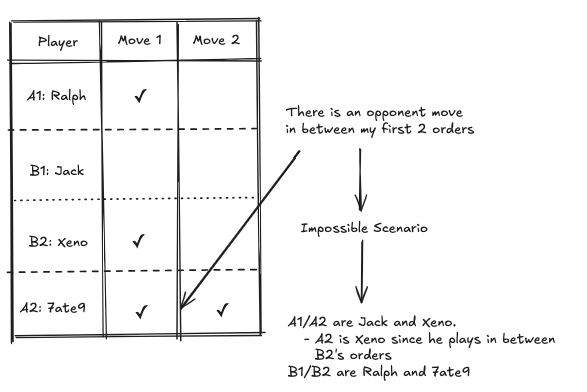
\includegraphics[width=0.7\textwidth]{Images/2v2figuring.jpg}
  \caption{Deriving move order}
  \label{2v2deriving}
\end{figure}

Following the same \href{https://www.warzone.com/MultiPlayer?GameID=37917076}{Strategic 2vs2} game, after figuring the Move Order, the next step is utilizing that so as to get any information possible for the opponent spawns as well as expansion and leftover armies.

\paragraph{2vs2: ABBA in making picks: Mirroring}

In a Game between 2 teams, A and B, with each team having x number of players and each player receiving y number of territories, the total number of territories allocated to all players participating is \textit{2xy}. As such, during pick phase, you should always make enough picks up to the number \textit{2xy}, as you might end up losing enough picks to reach that number.
\\
\\
There is a core idea behind picking in Team Games, that holds true to every Team Game, regardless of the amount of players participating, and that is mirror picking. Suppose that in a 2vs2 template, there as an undisputed best territory/bonus in the board and you want for your team (team A for the example's sake) to maximize the chances that you get that. If team B mirror picks (meaning both B1 and B2 put their first pick on that territory), whereas team A has only A1 first pick it, then Team A has 25\% probability to get first pick. Therefore, if there is a territory you want to make sure your team gets, mirroring first pick is the way. Expanding this idea to a quantifiable 2vs2 template where team A can confidently order the territories in distribution in a ranking of preference, has given birth to the idea that is "full mirroring".
\\
\\
By full mirroring, we refer to teams that would mirror pick their entire set of picks. For example, in Final Earth 2vs2 (commonly referred as Strat 2vs2) where each player receives 3 initial territories, full mirroring refers to making a ranking of 12 territories in the map and mirror picking the entire list. If a team full mirrors 1->12 in Final Earth 2vs2 and doesn't lose a single pick during pick phase, they get their first 6 territories, meaning player A1 receives 1,4,5 while A2 receives 2,3,6. If the team loses for example picks 3 and 4, then suddenly the distribution looks like A1: 1,6,7 and A2: 2,5,8 and the allocation looks completely different. This introduces us to the biggest drawback in mirror picking, that is ensuring coverage in the map for all possible scenarios of pick combinations for both players. Take a close look for example at this \href{https://www.warzone.com/MultiPlayer?GameID=39930222}{CW 2vs2} game. Team A full mirrors and receives their 1,3,4,6,7,8 allocated as:
\begin{itemize}
    \item Aika: 1,6,7
    \item No.One: 3,4,8
\end{itemize}
After Turn 1 we quickly see that Aika has 3 contested picks. In expansion-heavy 2vs2 templates that might not be a big issue, as long as No.One could expand while Aika absorbs pressure, but 3 fronts vs 2 opponents at Turn 2 is impossible to overcome. 
\\
\\
The argument in favor of mirroring (not necessarily full mirroring), is reducing the degrees of freedom or variance during picking phase. For example, take a look at this \href{https://www.warzone.com/MultiPlayer?GameID=38651245}{Ladder 2vs2} game, accompanied by Figure \ref{abba2v2}. In the Figure, I have denoted:
\begin{itemize}
    \item With G10 the 5 wastelands as well as with T2 the neutrals in the bonuses containing wastelands and R4 the in distribution spawns that belong to wastelanded bonuses.
    \item With Y4 the pickable territories in distribution.
    \item With white regions the 5 income zones. Thick white lines for the 2 safest income regions, Africa and Oceania, with the other 3 for NA, SA and Eurasia.
    \item With Yellow Team A's picks.
    \item With Pink Team B's picks.
    \item With Black arrows the fastest paths into the safe regions.
    \item With Bright Green 2 important territories in Eurasia.
\end{itemize}

\begin{figure}[H]
  \centering
  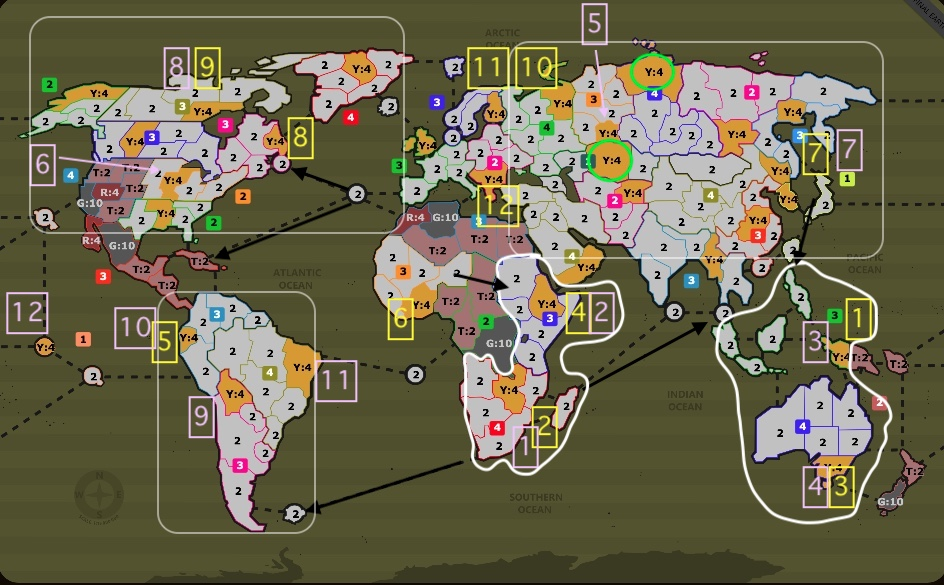
\includegraphics[width=0.95\textwidth]{Images/abba2v2.jpg}
  \caption{Map dynamics of this distribution}
  \label{abba2v2}
\end{figure}

First things first we can spot that both teams decide on covering the 2 safest income regions at picks 1-4 with the reasons being:
\begin{itemize}
    \item If we successfully get our first 4 picks, with our last 2 picks as a team we cover 2/3 of the large income regions within 1-3 turns. The paths should be obvious: 
    \begin{itemize}
        \item Indonesia -> Japan -> Cover East Asia
        \item Oceaania -> Hawaii -> Cover USA
        \item South Africa -> Argentina -> Cover SA
        \item East Africa -> Europe into West Russia
    \end{itemize}
    \item If we get 3 out of our first 4 picks, this means we have secured 1 safe income region and opt to get coverage in the other 3.
    \item If we split both safe income regions (expected result), we have to optimize accordingly the later picks.
\end{itemize}

\begin{wrapfigure}{r}{0.5\textwidth}
    \centering
    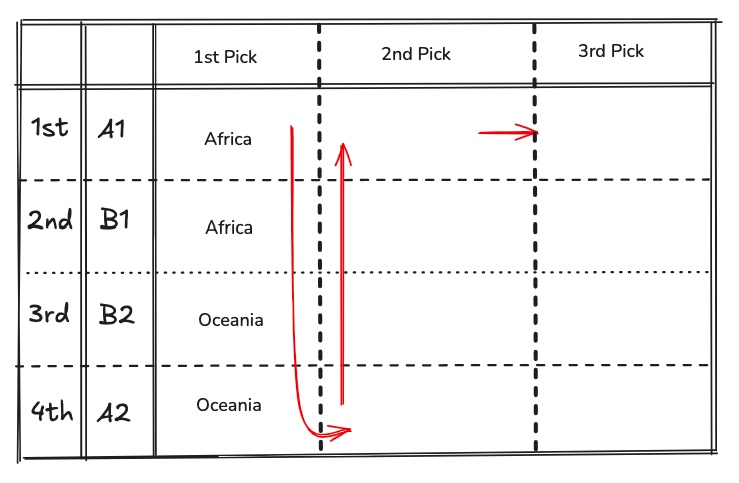
\includegraphics[width=0.45\textwidth]{Images/opt2v2.jpg}
    \caption{ABBA if we split 1-4}
    \label{opt2v2}
\end{wrapfigure}
But what does it mean to optimize later picks? Under those premises, player A2 will get a territory, followed by team A getting 2 consecutive territories. So, if I am making picks and expecting my opponents to go for the same 1-5 territories, if I cover a region only with my 5th pick, I risk a 50-50\% chance of losing that territory. If I want to take that risk I must optimize my 6/7, as I will be guaranteed to get them.
\\
\\
With that settled, the my pickset now make more sense.
\begin{enumerate}
    \item For my picks (7ate9): I select 5th in Ural based on:
    \begin{enumerate}
        \item It's 3 double borders are all 4army neutrals that I either see Turn 1 or Turn 2 -> is relatively safely
        \item It is in the center of the biggest income region on the map, eurasia.
        \item Has immediate expansion if needed. 
        \item Is a +3 bonus. Since I expect early contact and splitting 1-4, it's generally better to go for safe +3 bonuses instead of +4, as +4s require 10/10 of your deployments in the first 2 turns.
    \end{enumerate}
    \item If I lose Ural, I always get 6/7, which ensures for me coverage on NA and a backup safe +3 bonus in eurasia, Fast East Russia. The latter is especially useful for having direct paths to Oceania and NA.
    \item If I lose 6 in NA I either get two picks from 1-4, 5,7,8 and a last one, or I am getting two from 1-4, 5,7,9 and 1 more. Notice that it is impossible to lose all 6,7,8 under this scenario of splitting 1-4. As such,
    \begin{enumerate}
        \item If I get two from 1-4, 5, 7, 8 and a last one, 8 is my coverage for NA and with the remaining picks i can stack cover the last income region.
        \item If I get two from 1-4, 5,7,9 I should be team A, have lost 6,8 but have Far East Russia to cover NA if needed + position my 10 in SA in the spawn closest to NA, while 12 also can positionally cover that.
    \end{enumerate}
\end{enumerate}

\paragraph{2vs2: ABBA in making picks: Not Mirroring}

As some wise people have said, full mirroring is a lazy way to pick. Let's take a look at two games, with the first one this \href{https://www.warzone.com/MultiPlayer?GameID=38757694}{Biomes 2vs2} game. 

\begin{wrapfigure}{r}{0.5\textwidth}
    \centering
    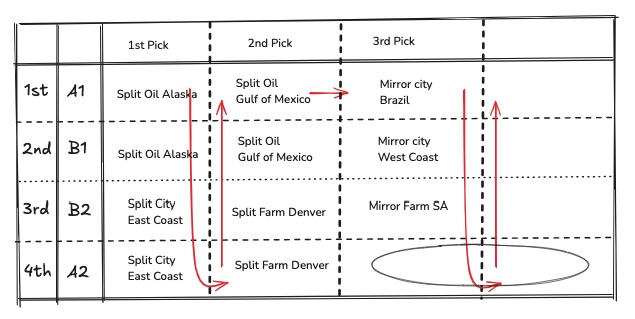
\includegraphics[width=0.5\textwidth]{Images/boa2v2.jpg}
    \caption{ABBA in Biomes 2v2, 1}
    \label{boa2v2}
\end{wrapfigure}

Upon looking at the distribution there are 3 combos that can either net income turn 1 or +3/+4 income on turn 2 with 0 deployments, followed by the more niche but equally strong combo in Gulf of Mexico. Due to the other good picks being relativelly slow, with the exception of the city in Brazil which can be covered in multiple ways, let's accept that the best course of action is split picking the 4 combos from 1-4 in both players. After that, Team A has a guaranteed pick on player A1, followed by two picks for team B followed by two picks on player A2. 
\\
\\
The key in this distribution is recognizing that there are 3 territories worth mirroring at 5-7, in two cities and the farm in SA (look Rufus' team picks). If he loses the city in Brazil, he guarantees 6,7 which provide the last city as well as the farm in Argentina. Even more importantly, 8/9 should be split picks, since if you are team A, you want to capitalize on the fact that A2 will get two picks consecutively and you want to aim at them getting initial income.
\\
\\
In another example, again at \href{https://www.warzone.com/MultiPlayer?GameID=38696110}{Biomes 2vs2}:

\begin{wrapfigure}{r}{0.5\textwidth}
    \centering
    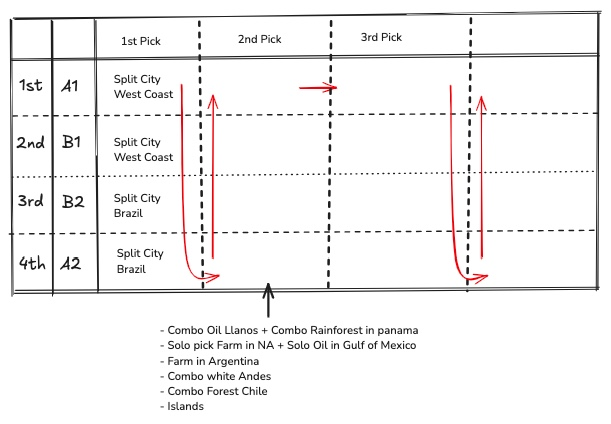
\includegraphics[width=0.5\textwidth]{Images/boarps.jpg}
    \caption{First 4 picks}
    \label{boarps1}
\end{wrapfigure}

There are in the distribution two undisputed busted city combos that both teams should split pick 1-2 otherwise they are completely trolling. But after that we have a problem, as there are so many different combos and individual territories that we would like to cover. Experienced players should agree that the combo in Llanos (oil) as well as the solo Farm pick in NA are the best of the rest, as we can make multiple picks around Argentina and the whites in the surrounding region to ensure coverage. If we proceed on split picking after 1-2 and have one player do 3 in Farm in NA and 4 onward somewhere in Argentina while the other player does 3/4 in the oil in Llanos, then there is a hidden trap, that I try to exploit with my pickset.
\begin{itemize}
    \item If the 3/4 Oil player is A1 and team B mirror picks 3-5 (2x Oil and Farm), then A2 gets solo Farm and team B get both Oil picks and can gift Turn 1 to get the bonus. Therefore there is 25\% chance that a team not mirroring 3-5 can lose that combo entirely.
\end{itemize}

Proceeding on the same path, there are more issues arising, as shown in \ref{boarps2}. 
\begin{wrapfigure}{r}{0.5\textwidth}
    \centering
    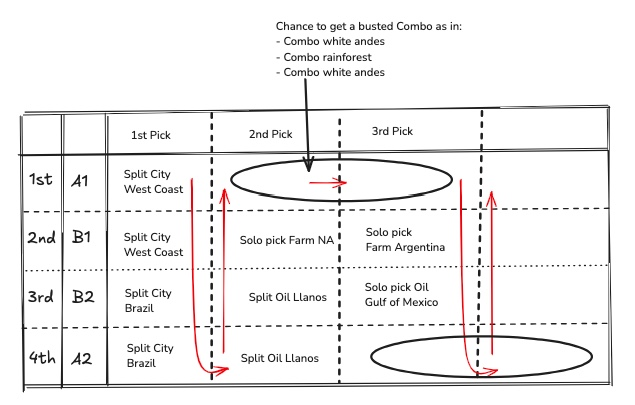
\includegraphics[width=0.5\textwidth]{Images/boarps2.jpg}
    \caption{Later picks}
    \label{boarps2}
\end{wrapfigure}

As long as both teams in some way or another split all picks from 1-7, player A1 is about to get a combo, with 2 consecutive picks. So, the correct approach after the combo oil \& farm in NA, is to split pick between the two players of the team for the combos in either the rain-forest, or forest, or whites, so as to ensure that if you are team A, you get a really good combo on A1. Then, the only compensation that team B can get, since B1 and B2 get a pick each, and not a combo in one of them, is the Farm in Argentina as well as the Oil in Gulf of Mexico, followed by a combo pick for player A2.

Understanding all the intricacies of ABBA will give you the upper hand and a better and thorough understanding of the picking phase.

\subsubsection{3vs3}

Similarly to 2vs2 games, 3vs3 also tend to have cyclic move order. Expanding on this, the order follows the same ABBA pattern. In a 3vs3 game between Team A (players A1, A2 and A3) and Team B (players B1, B2 and B3), the move order would follow the pattern $$\text{A1,B1,B2,A2,A3,B3} ,\text{B3,A3,A2,B2,B1,A1} , \text{A1,B1,B2,A2,A3,B3} \dots$$

This is best illustrated in the Figure \ref{3vs3}. Also remember that the ABBA pattern follows both the moves - orders and the deployments.

\begin{figure}[H]
  \centering
  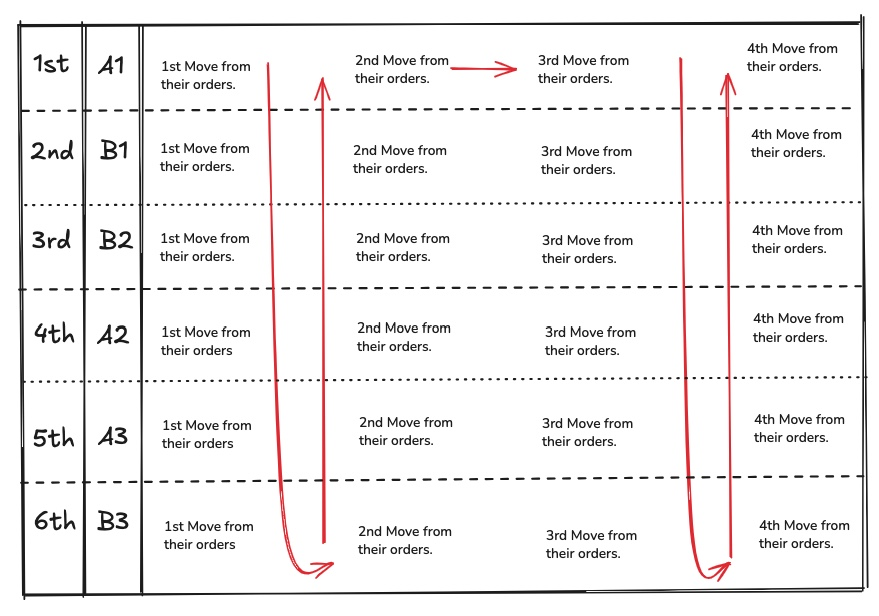
\includegraphics[width=0.8\textwidth]{Images/3vs3.jpg}
  \caption{ABBA in moves in 3vs3}
  \label{3vs3}
\end{figure}

Mirroring, either fully or partially is extremely common in non-INSS 3vs3 templates, as it drastically reduces the number of variables while at the same time optimizing the probabilities of certain cover or combo picks. For example, one can go into analysing in detail \href{https://www.warzone.com/MultiPlayer?GameID=33969282}{this CL 3vs3 game}, while taking into account \ref{3vs3alloc}, being the order of pick allocation during the game. Analyzing a 3vs3 Europe game is an a exhausting and complicated task, in which I will not delve into at the moment.

\begin{figure}[H]
  \centering
  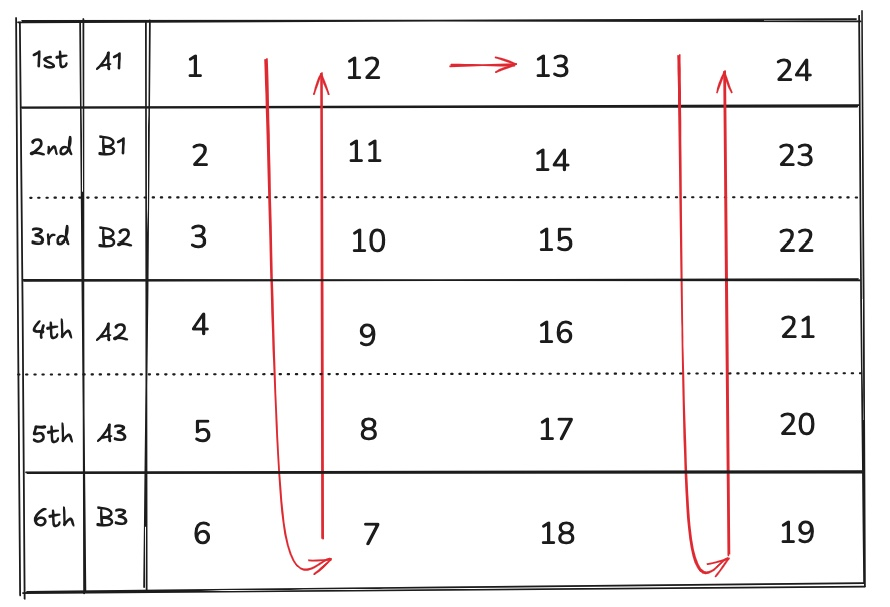
\includegraphics[width=0.8\textwidth]{Images/3vs3alloc.jpg}
  \caption{Order of pick allocation in 3vs3}
  \label{3vs3alloc}
\end{figure}
